\documentclass{myclass}

\begin{document}

\section{What is a neural network?}

History of neural networks dates back at least to the 1950s when F. Rosenblatt proposed the
perceptron model. The basic computational unit in such a network was the McCulloch--Pitts neuron
which realized the following mapping \(\Rbb^n \mapsto \Rbb\)
\[
\boxed
{
   f(\bm{x}) = \varphi \left( \bm{x} \bm{w}^\tpose + b \right)
}\,,
\]
where \(\bm{x} = \mqty[x_1 & \ldots & x_n]\) is the vector of input signals, \(\varphi\) is some
nonlinear activation function and \(\bm{w}\), \(b\) are some parameters (\(\bm{w}\) called the
weights and \(b\) called the bias). Multilayer perceptron was built from many such neurons connected
in layers so that the connections existed only between the neurons in neighboring layers and there
were no connections between the neurons in the same layer. 

\begin{figure}[ht]
   \centering
   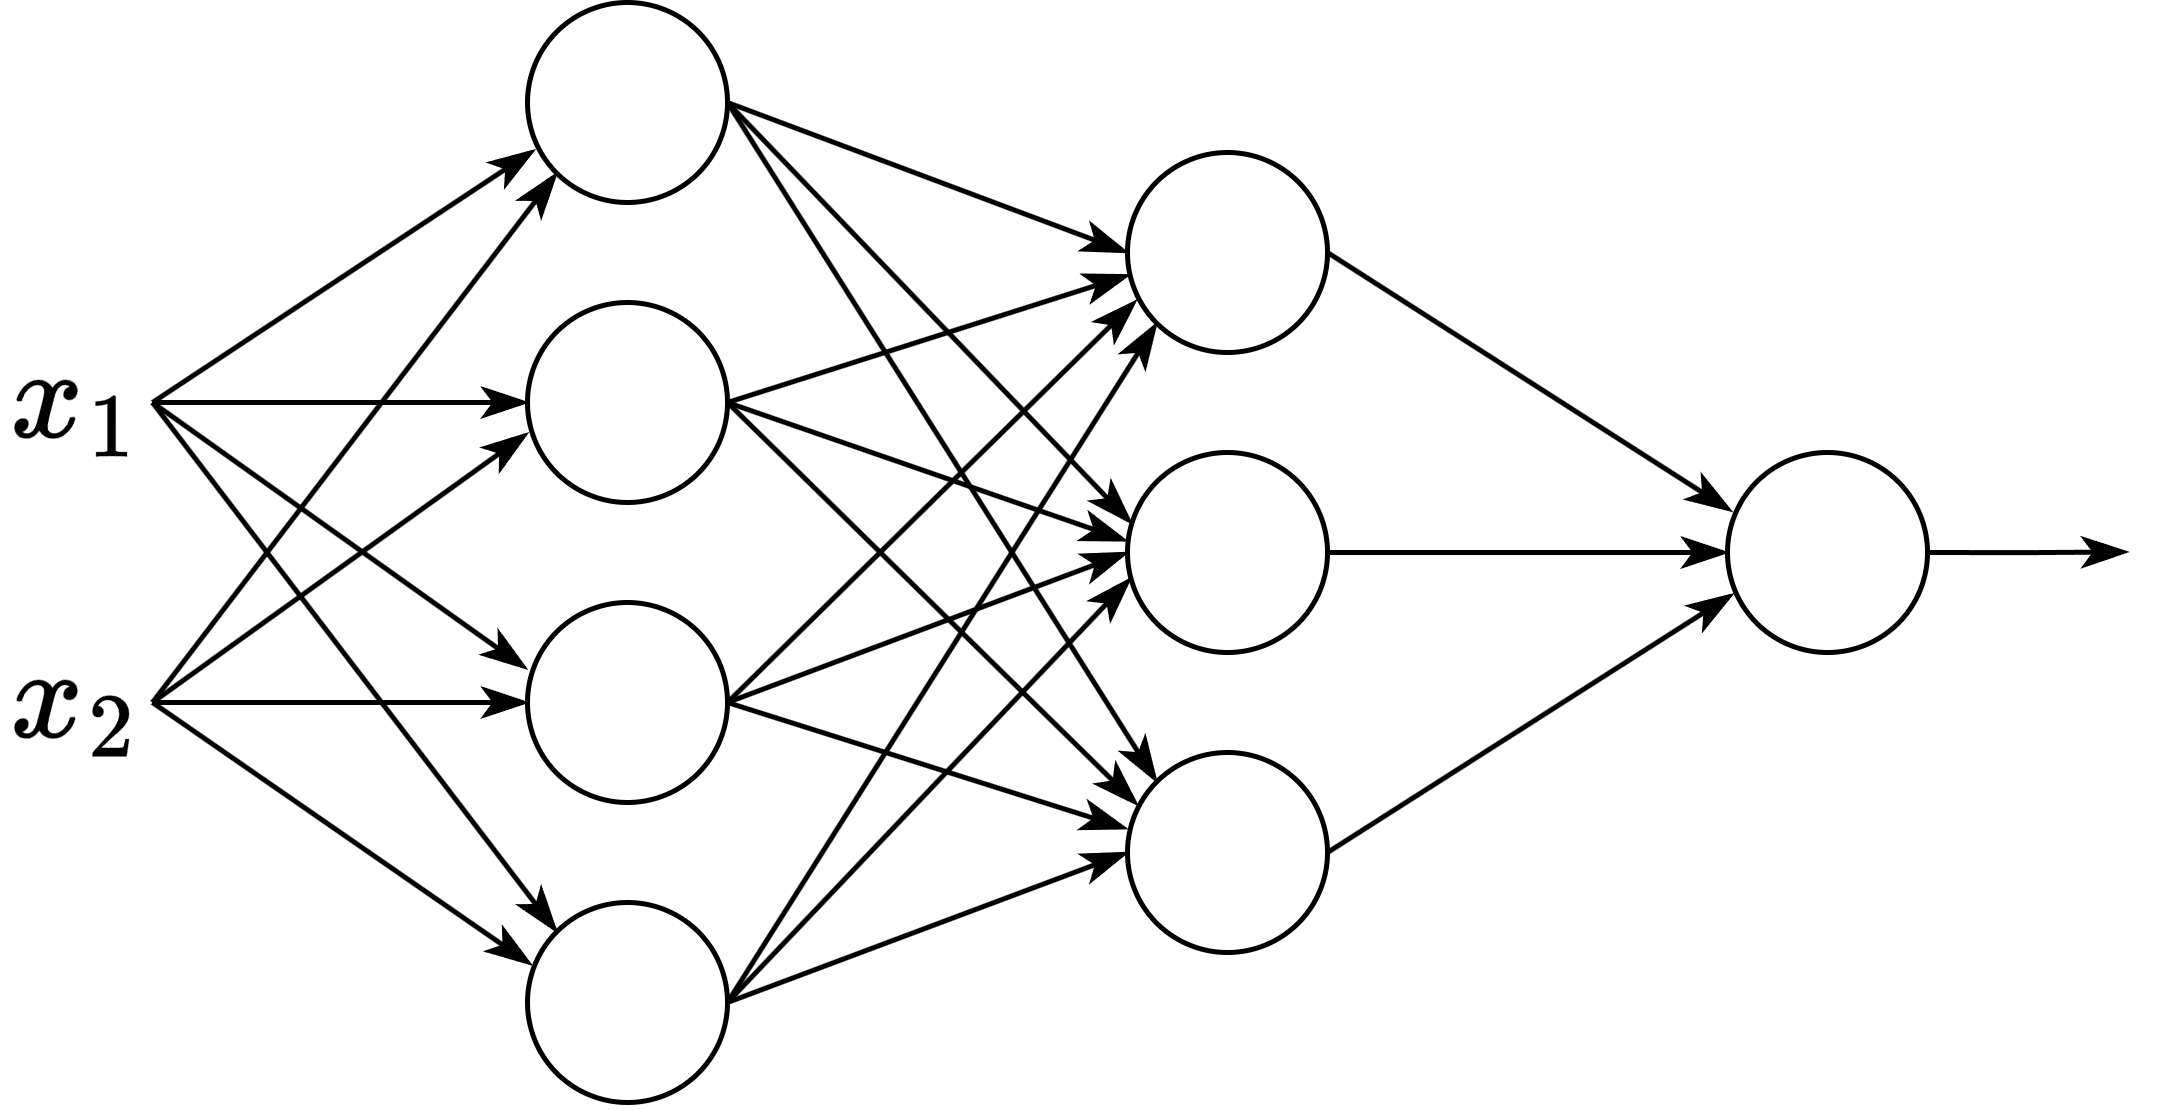
\includegraphics[width=0.85\columnwidth]{figs/nn.png}
\end{figure}

In general neural network is any Directed Acyclic Graph (DAG) in which every vertex \(i\) has the
following attributes.

\medskip

1. Set of previous vertices -- \(\mathscr{P}_i\).

\medskip

2. Set of next vertices -- \(\mathscr{N}_i\).

\medskip

3. Parametrized tensor function \(\bm{F}^{(i)}\) of the form
\[
   \Rbb^{\left(n_{1}^{(1)}, \ldots, n_{k_1}^{(1)}\right)} \times \ldots \times  \Rbb^{\left(n_{1}^{(p)}, \ldots, n_{k_p}^{(p)}\right)} \times \Theta \mapsto \Rbb^{(m_1, \ldots, m_l)}
\]
The function takes \(p\) tensor arguments of dimensions \(k_1,\ldots,k_p\) respectively (input
tensor \(q\) of dimension \(k_q\) has \(n_{r}^{(q)}\) elements along the \(r\) axis) and parameters
\(\bm{\theta}^{(i)} \in \Theta\) and returns a tensor of dimension \(l\). Obviously it must satisfy
\(p = |\mathscr{P}_i|\) and the tensors returned by the parent nodes must have appropriate shapes.

\medskip

4. The gradient functions of the function \(\bm{F}^{(i)}\) w.r.t. to the parameters and w.r.t. all
the inputs, that is for all \(j \in \mathscr{P}_i\) we have a gradient functions
\[
   \pdv{F_\beta ^{(i)}}{\theta_\alpha ^{(i)}}\,,\quad \pdv{F_\beta ^{(i)}}{F_\alpha ^{(j)}} \,,
\]
where \(\alpha\), \(\beta\) are the suitable multi-indices.


\section{Loss functions}

Training of a neural network consists of changing the parameters \(\bm{\theta}^{(i)}\) of the nodes
in such a way as to make the network perform the given task. The task is specified by a training set
\(\mc{X}\) which contains the ''blueprint answers'' of the network. To train the network we
introduce the quantitative measure of networks performance on the dataset which implicitly (through
the outputs of the network) depends on the parameters of the network (here collectively denoted by
\(\bm{\theta}\)) \(L(\mc{X}, \bm{\theta})\). Training can be then phrased as an optimization problem
of the form
\[
   \bm{\theta}^* = \arg \min_{\bm{\theta}} L(\mc{X}, \bm{\theta})
\]
for a fixed training set \(\mc{X}\).

\medskip

There is no single established way of constructing loss functions. One of the more motivated
approaches is based on the maximum likelihood criterion. The idea is that we model our data using
some parametrized statistical model and express the parameters of this model as an output of a
neural network. The loss function is then taken to be the \emph{negated log-likelihood function}. In
this manner one can derive the most common loss functions.


\subsection{Mean Squared Error}

\[
\boxed{ L(\mc{X}, \bm{\theta}) = \frac{1}{n} \sum_\alpha \left[ y_\alpha - \Phi_\alpha(\bm{X};\bm{\theta}) \right]^2}
\] 
where \(\bm{X}\) is a tensor which can be interpreted as a stack of \(n\) 1-D feature-vectors
residing in the last dimension of \(\bm{X}\), \(\bm{y}\) is the corresponding tensor of \(n\) scalar
continuous outputs for each feature-vector (so called target) and \(\bm{\Phi}\) denotes the neural
network.


\subsection{(Binary) Cross Entropy}

\[
\begin{split} 
   &\boxed{L(\mc{X}, \bm{\theta}) = \frac{1}{n} \sum_{\alpha} \left[ t_\alpha \log\pi_\alpha + (1-t_\alpha)\log(1-\pi_\alpha) \right]} \\
   &\bm{\pi} = \sigma\left( \bm{\Phi}(\bm{X}; \bm{\theta})\right)\,,\quad \sigma(z) = \frac{1}{1 + \e^{-z}}\,,
\end{split}
\] 
where \(\bm{X}\) is a tensor which can be interpreted as a stack of \(n\) 1-D feature-vectors
residing in the last dimension of \(\bm{X}\), \(\bm{t}\) is the corresponding tensor of \(n\) binary
(i.e. 0 or 1) values denoting the class for each feature-vector, \(\sigma\) is the logistic
function, \(\bm{\Phi}\) denotes the neural network and \(\bm{\pi}\) is a tensor of the same shape as
\(\bm{t}\) which contains the probabilities of the positive class.


\subsection{Cross Entropy}

\[
\begin{split} 
   &\boxed{L(\mc{X}, \bm{\theta}) = \frac{1}{n}\sum_{\alpha}\sum_{\beta} t_{\alpha\beta} \log \pi_{\alpha\beta}}\\
   & \bm{\pi} = \bm{\sigma}\left( \bm{\Phi}(\bm{X};\bm{\theta}) \right)\,,\quad \sigma_{\alpha'\alpha}(\bm{z}) = \frac{\exp z_{\alpha'\alpha}}{\sum_{\beta} \exp z_{\alpha'\beta}}\,,
\end{split}
\] 
where \(\bm{X}\) is a tensor which can be interpreted as a stack of \(n\) 1-D feature-vectors
residing in the last dimension of \(\bm{X}\), \(\bm{t}\) is the corresponding thensor which can be
interpreted as a stack of \(n\) 1-D one-hot-vectors residing in the last dimension of \(\bm{t}\)
encoding the correct class, \(\bm{\sigma}\) is the soft-max function which given the stack of 1-D
vectors independently normalizes each of them so that the entries are non-negative and sum to 1 and
\(\bm{\Phi}\) denotes the neural network.


\section{Forward propagation}

Let \(\bm{v}^{(i)}\) be the (tensor) value of the function \(\bm{F}^{(i)}\). To propagate the
(tensor) inputs to the network and get the output we use the following recursive equation
\[
\boxed{ \bm{v}^{(i)} = \bm{F}^{(i)} \left[ \left(\bm{v}^{(j)}\right)_{j \in \mathscr{P}_i} ; \bm{\theta}^{(i)} \right] }'
\] 
and visit the nodes in the \emph{topological order} as this guarantees that we visit every node
exactly once. We assume here that nodes \(\bm{v}^{(i)}\) such that \(\mathscr{P}_i = \varnothing\)
are the inputs to the network and nodes \(\bm{v}^{(i)}\) such that \(\mathscr{N}_i = \varnothing\)
are the output of the network.


\section{Backward propagation}

Let \(L\) be the loss function. In order to compute the derivatives
\(\partial_{\bm{\theta}^{(i)}}L\) we use the following recursive equations
\[
\boxed{
\begin{split} 
   &\pdv{L}{\theta^{(i)}_\alpha} = \sum_\beta \pdv{L}{F^{(i)}_\beta} \pdv{F^{(i)}_\beta}{\theta^{(i)}_\alpha} \\
   &\pdv{L}{F_\alpha^{(i)}} = \sum_{j \in \mathscr{N}_i} \sum_\beta \pdv{L}{F_\beta^{(j)}} \pdv{F_\beta ^{(j)}}{F_\alpha^{(i)}}
\end{split}
}
\] 
where \(\alpha\), \(\beta\) are the suitable multi-indices. We visit nodes in the \emph{reversed
topological order} and compute and store the values of loss function derivatives. All derivatives
are computed for the current values of \(\bm{v}^{(i)}\) and \(\bm{\theta}^{(i)}\), therefore before
backward propagation one must perform forward propagation to compute values \(\bm{v}^{(i)}\).


\section{Stochastic Gradient Descent}

The standard optimization method used to train neural networks is the Stochastic Gradient Descent,
which is an iterative, gradient-based algorithm in which in every step \(t\) we update the
parameters \(\bm{\theta}^{(i)}\) utilizing the gradient information. Let \(\bm{\theta}^{(i,t)}\)
denote the value of parameters \(\bm{\theta}^{(i)}\) at step \(t\) and let \(\bm{v}^{(i,t)}\) be the
values of the function \(\bm{F}^{(i)}\) at step \(t\). In each step we take a batch \(\mc{X}\)  of
training data, perform forward propagation to compute values \(\bm{v}^{(i,t)}\) and the value of the
loss function \(L(\mc{X},\bm{\theta}^{(t)})\), next perform backward propagation to compute the
values of gradients \(\bm{g}^{(i,t)} =
\partial_{\bm{\theta}^{(i)}}L\left(\mc{X},\bm{\theta}^{(t)}\right)\) and afterwards we update the
parameters according to
\[
   \boxed{ \theta_\alpha^{(i,t+1)} = \theta_\alpha^{(i,t)} - \eta g_\alpha^{(i,t)} }
\] 
where \(\eta\) is the learning rate.


\subsection{Momentum}

The problem with vanilla SGD is that it gets stuck in the local minima. To overcome this problem one
can take inspiration from simple physics. We first introduce velocity tensor \(\bm{V}\) with the
following update rule
\[\boxed{ V^{(i,t+1)}_\alpha = \gamma V^{(i,t)}_\alpha - \eta g^{(i,t)}_\alpha }\] where \(0 <
   \gamma < 1\) is the so called momentum term and update parameters using
\[\boxed{ \theta_\alpha ^{(i,t+1)} = \theta_\alpha ^{(i,t)} + V_\alpha ^{(i,t+1)} }\]


\subsection{Adaptive Moment Estimation (Adam)}

Another problem with vanilla SGD is that it uses the same learning rate for every scalar parameter.
Adam algorithm solves this problem by introducing running averages with exponential forgetting of
both the gradients and the second moments of the gradients.
\[
\boxed{
\begin{split} 
   &M_\alpha^{(i,t+1)} = \beta_1 M_\alpha^{(i,t)} + (1-\beta_1) g_\alpha^{(i,t)} \\
   &V_\alpha ^{(i,t+1)} = \beta_2 V_\alpha^{(i,t)} + (1 - \beta_2) \left(g_\alpha^{(i,t)}\right)^2\\
   &\tilde{M}_\alpha^{(i,t+1)} = \frac{M_\alpha^{(i,t+1)}}{1 - \beta_1^t} \\
   &\tilde{V}_\alpha^{(i,t+1)}=\frac{ V_\alpha^{(i,t+1)}}{1 - \beta_2^t} \\
   &\theta_\alpha ^{(i,t+1)} = \theta_\alpha ^{(i,t)} - \eta \frac{\tilde{M}_\alpha^{(i,t+1)}}{\sqrt{\tilde{V}_\alpha^{(i,t+1)}} + \epsilon}
\end{split}
}
\] 
where \(\epsilon \simeq 10^{-8}\)  is used to prevent division by 0, \(\eta\) is the learning rate
and \(\beta_1\) and \(\beta_2\) are the forgetting factors typically set to \(\beta_1=0.9\) and
\(\beta_2=0.999\). Additionally popular choice for \(\eta\) is \(\eta = 3\cdot10^{-4}\).


\subsection{Asynchronous SGD}

...


\section{Regularization}

Neural networks have very high capacity, meaning they are very flexible and can easily overfit.
Regularization methods are methods used to fight this phenomenon.


\subsection{Weight decay}

Weight decay is a simple regularization method present already in classical, shallow machine
learning models, in which we simply add to the loss function a suitably chosen norm of the
parameters of the model
\[
   L^*(\mc{X}, \bm{\theta}) = L(\mc{X}, \bm{\theta}) + \lambda \norm{\bm{\theta}}_p^p\,.
\]
Typically one uses the L1 or L2 norms (\(p=1,2\)). The most important difference between the two is
that L1 norm contains implicit feature selection that is it often makes the parameters exactly 0,
while L2 norm only encourages the weights to be values close to 0. 


\subsection{Weight normalization}

The problem with weight decay is that each parameter is limited independently of others. Weight
normalization is a regularization technique that forces the weights to ''compete'' against each
other so that only the most important parameters remain. The idea is following, we introduce the
limit for the norm of weight vector \(\ell\). After each parameter update, we compute the vector
\(p\)-norm
\[
   N_{\alpha} = \left( \sum_{\beta} \left|\theta_{\alpha\beta}\right|^p \right)^{1/p}
\]
and update the weights according to
\[
   \theta_{\alpha\beta} \gets \begin{cases} 
                           \theta_{\alpha\beta}                            &\text{ if \(N_\alpha \leq \ell\)}\\
                           \frac{\ell}{N_\alpha} \theta_{\alpha\beta}   &\text{ if \(N_\alpha > \ell\)}
   \end{cases}\quad.
\]


\subsection{Early stopping}

The simplest, yet extremely powerful and popular form of regularization is the early stopping. The
idea is that we divide the training set into a smaller training set and a validation set. We train
the model on this smaller training set and at the same time measure the performance of the model on
the validation set. If the loss gets smaller on both of these sets, everything is alright, but the
moment the loss on the validation set starts rising, while the loss on training set gets smaller we
stop the training, as this means the model is starting to overfit.


\subsection{Dropout}

A general method of regularization of any machine learning model is averaging the answers of an
ensemble of similar models trained on different subsets of the training set which make different
mistakes. The naive implementation of this method for the neural networks is not feasible as neural
networks require vast computational resources in the training process. The method which effectively
realizes this ensembling is dropout. The idea is to introduce layers into the computation graph
which during training multiply the inputs elementwise by a binary tensor whose element can be 0 or 1
with specified probability \(p\). During training, in each forward pass we sample such tensor and
update the running sum. Having finished training we normalize the running sum tensor (i.e. divide it
by the number of forward passes in training phase) and during forward pass multiply by it.


\subsection{Transfer learning}

When training data are limited, other datasets can be exploited to improve performance. In transfer
learning, the network is pre-trained to perform a related secondary task for which data are more
plentiful. The resulting model is then adapted to the original task. This is typically done by
removing the last layer and adding one or more layers that produce a suitable output. The main model
may be fixed, and the new layers trained for the original task, or we may finetune the entire model.
The principle is that the network will build a good internal representation of the data from the
secondary task, which can subsequently be exploited for the original task. Equivalently, transfer
learning can be viewed as initializing most of the parameters of the final network in a sensible
part of the space that is likely to produce a good solution.


\subsection{Augmentation}

Training set augmentation is a method of implicitly specifing certain invariances of the network by
modyfing the examples from the training set before feeding them into the network. Typical examples
are image transformations for convolutional neural networks trained to classify images as we want
the output of the network to be invariant under rotations, zoom, reflection, etc.


\section{Initialization}

One important aspect of neural networks is the way we initialize the parameters before training.
Since the neural network effectively realizes a highly nonlinear mapping, the loss as a function of
the parametrs is also highly nonlinear and non-convex. Because of this the initial values of the
parameters do matter. The simplest form of initialization is zero initialization in which we just
set \(\theta = 0\). This however leads to too much symmetry and thus we almost always use random
initialization in which we sample weights (independently) from some probability distribution --
typically uniform distribution centered at 0 with small width e.g. \(\pm0.005\) or normal
distribution with mean 0 and small variance like \(0.01\). Several authors proposed more specific
initialization schemes (typically for fully connected layers) based on analysis of the variance of
activations between the layers. Assuming \(n_i\) and \(n_{i+1}\) are the number of neurons
(dimensions of outputs) in subsequent layers we have the following.

\begin{itemize}
   \item \textbf{LeCun initialization.} We sample the weights from
   \[
      \mc{U}\left(-\sqrt{3n_{i}^{-1}}, +\sqrt{3n_{i}^{-1}}\right) \quad.
   \]
   This initialization is designed to preserve the variance of activations during the forward pass.
   
   \item \textbf{(Xavier) Glorot initialization.} We sample the weights from
   \[
      \mc{U}\left(-\sqrt{6(n_{i} + n_{i+1})^{-1}}, +\sqrt{6(n_{i} + n_{i+1})^{-1}}\right) \quad.
   \]
   This initialization is designed as a compromise between preserving the variances of activations
   during the forward pass and gradient variances during the backward pass.
   
   \item \textbf{(Kaiming) He initialization.} We sample the weights from \(\mc{N}\left(0, \sqrt{2
   n_{i}^{-1}}\right)\). This initialization is a modification of Xavier initialization for ReLU
   (Rectified Linear Unit) activation function
   \[\boxed{
      \text{ReLU}(z) = \max(0, z)
   }
   \]
   instead of previously used sigmoid activations.
\end{itemize}

Additionally there are methods called normalization methods whose aim is to reduce the need for
careful initialization, so that the neural networks have reasonable convergence for any sensible
initialization e.g. \(\mc{N}(0,0.01)\).


\section{Normalization}

\section{Architectures}

\subsection{MLP}
\subsection{RBM}
\subsection{DBN}
\subsection{CNN}
\subsection{Autoencoder}
\subsection{VAE}
\subsection{GAN}
\subsection{DDPM}
\subsection{Transformer}

\section{Interpretability}
\end{document}